\chapter{Path Plananing}\label{chap:Planning}

\section{Usage of the RRT* Vertices}

As shown in chapter \ref{sec:trajectory} it is possible to optimize a trajectory which passes through predefined vertices. From now on, the vertices are no longer chosen manually but are defined by the result of the RRT* algorithm. The computational efficiency of the RRT* algorithm combined with the positive features of the nonlinear optimization discussed in section \ref{sec:nonlinearopt} lead to a optimized trajectory in densely packed environment.

\subsection{Vertex Extension}


Since the RRT* algorithm does not consider the dynamical behavior of a UAV there are still some challenges converting the RRT* straight line solution into a polynomial trajectory. In other words, there is the possibility that the polynomial trajectory passing through the vertices of the collision-free straight line solution is in collision with an obstacle. In this case a vertex, which is located on the straight line, has to be added. \newline

The process of generating a collision-free optimized trajectory can be summarized in following steps:


\begin{enumerate}
  \item Generate a collision-free straight line solution using the RRT* algorithm
  \item Create an initial trajectory passing through the vertices of the straight line solution
  \item If the initial solution is in collision, extend the existing vertices by a vertex located on the straight line solution. Repeat this step until the trajectory is collision-free
\item Perform a nonlinear optimization on the collision-free trajectory
\item If the optimized solution is in collision, extend the existing vertices by a vertex located on the straight line solution and restart the nonlinear optimization. Repeat this step until the optimized trajectory is collision-free
\end{enumerate}

This schematic description of the process is depicted step by step in the subsequent figures for a better understanding.

\subsubsection{Generate a collision-free straight line solution using the RRT* algorithm.}

Figure \ref{pic:RRTstepOne} depicts the straight line solution of the RRT* algorithm, which is explained in section \ref{sec:RRTstar}.  The $\gamma$ parameter, which is needed to calculate the radius $r$ in equation \ref{equ:ballradius}, is set to $\gamma = 1.5$. Furthermore, the side length of the bounding box is set to $0.5m$ for each dimension. Although the hight of a UAV is commonly smaller than the length and the width this is required if great roll and pitch angles are permitted. \newline


Please note that, due to the randomness of the RRT* algorithm, the straight line solution depicted in figure  \ref{pic:RRTstepOne} is different than the straight line solution depicted in figure \ref{pic:bbx} even though the parameters are the same. 

\begin{figure}[h]
   \centering
   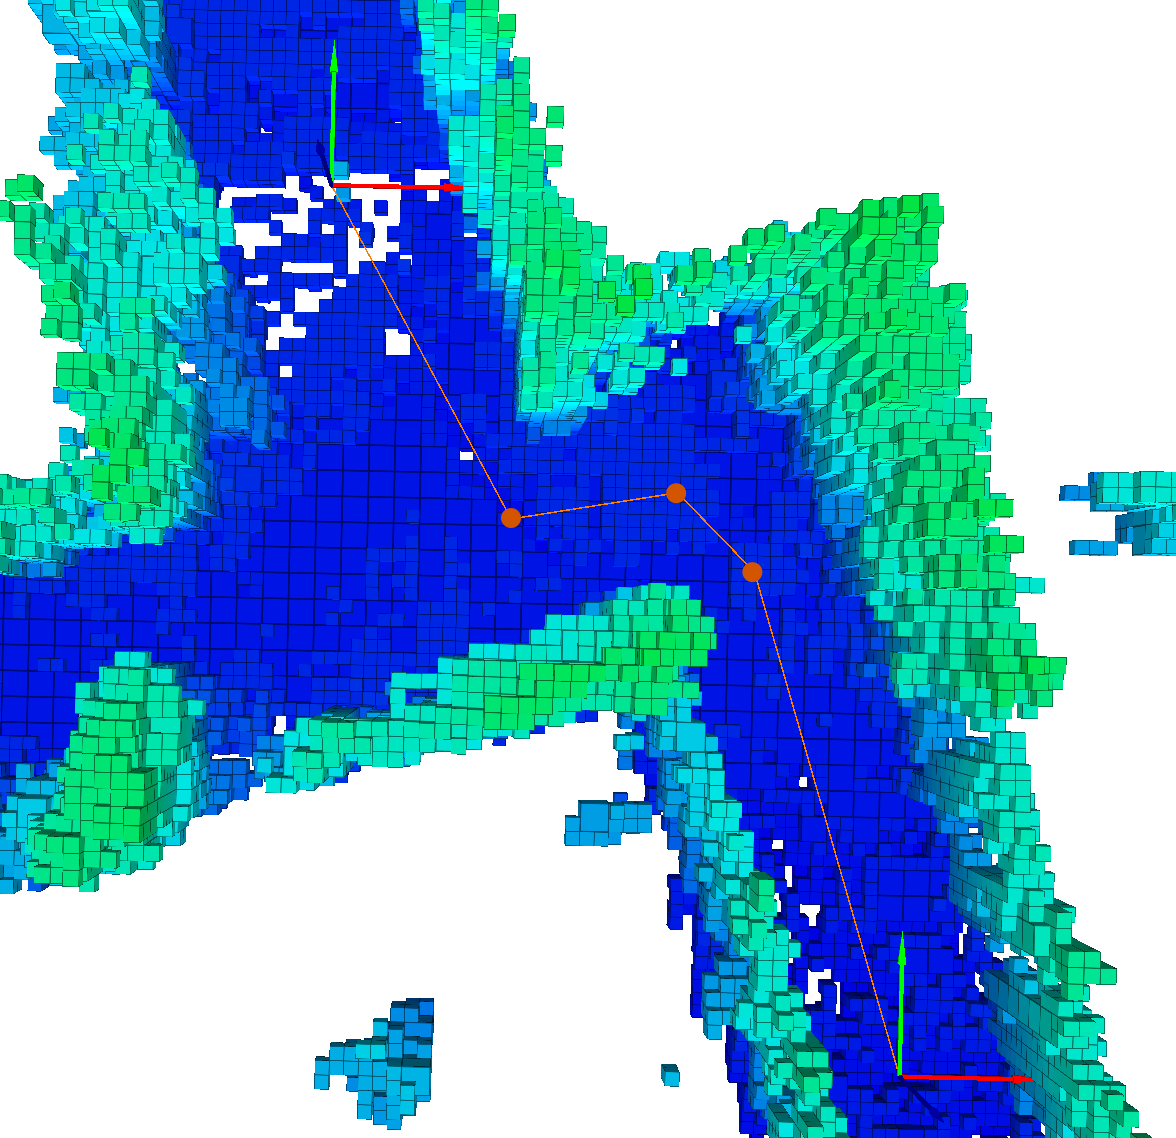
\includegraphics[trim = 45mm 0mm 35mm 0mm,clip,width=1\textwidth]{pics/extensionLongP.png}
   \caption{A collision-free straight line solution with 4 segments.}
   \label{pic:RRTstepOne}
\end{figure}


\subsubsection{Create an initial trajectory passing through the vertices of the straight line solution.}

The start and goal vertex (each marked by a red and green arrow in figure \ref{pic:RRTstepOne}) as well ass the 3 vertices (each marked by a orange dot in figure \ref{pic:RRTstepOne}) defined by the solution of the RRT* algorithm are now used to generate the initial polynomial solution according to equation \ref{equ:dpstar} and equation \ref{equ:segmentTime}. \newline

The initial trajectory passing through the vertices of the RRT* algorithm is depicted in figure \ref{pic:RRTstepTwo}. In the second segment there is a collision between the trajectory and the wall of the hallway (represented by green boxes). 



\begin{figure}[h]
   \centering
   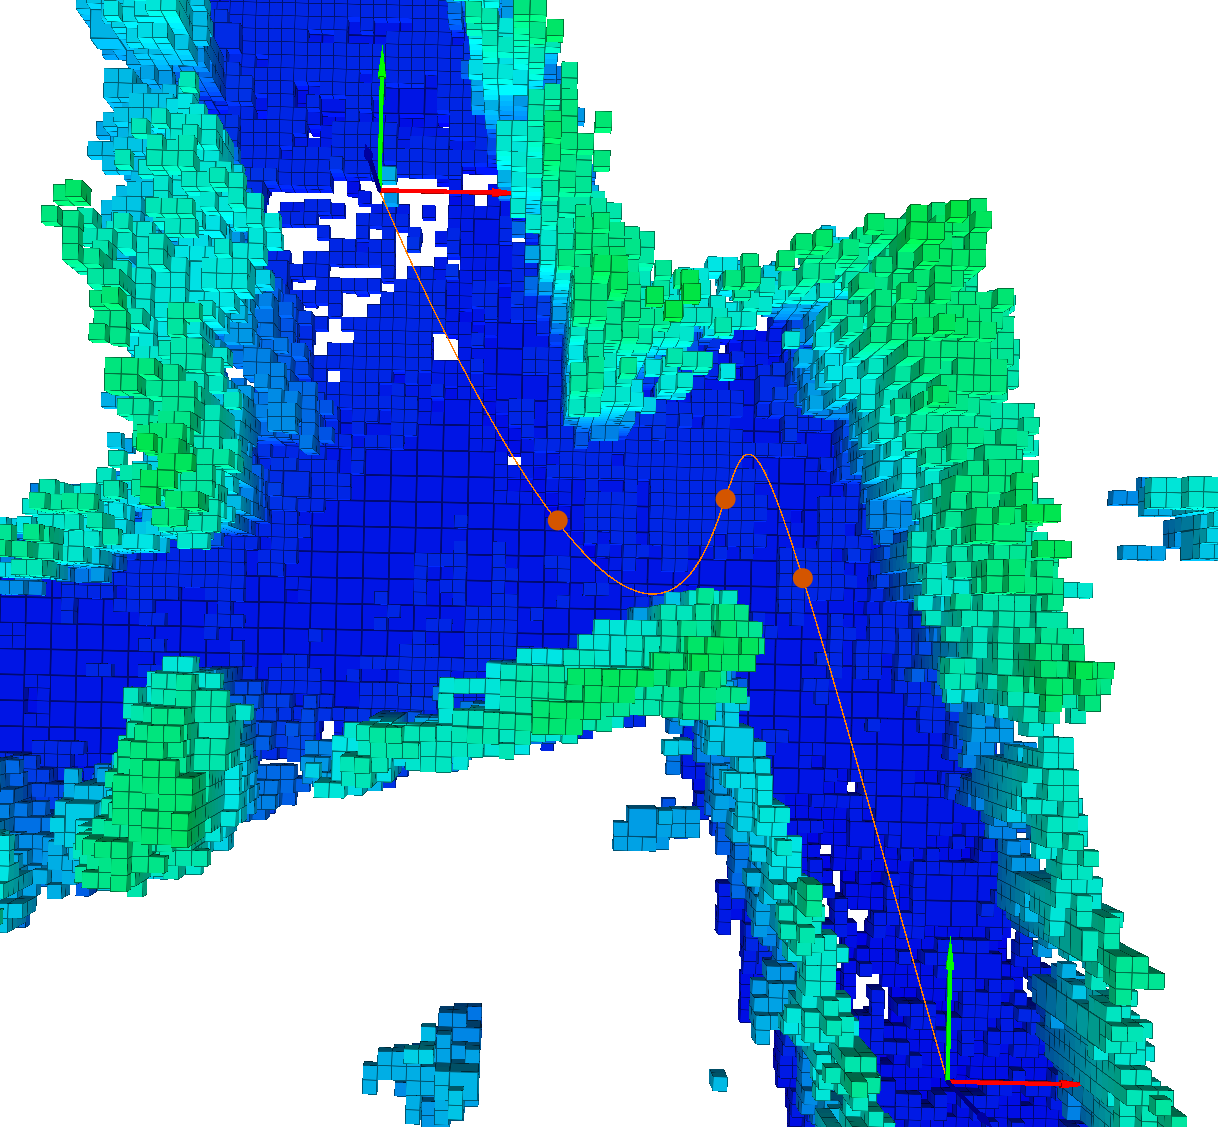
\includegraphics[trim = 45mm 0mm 35mm 0mm,clip,width=1\textwidth]{pics/extensionALongP.png}
   \caption{Initial trajectory with 4 segments. The start vertex is located in the upper left corner and the goal vertex is located in the lower right corner. There is a collision in the second segment of the trajectory.}
\label{pic:RRTstepTwo}
\end{figure}

\subsubsection{If the initial solution is in collision, extend the existing vertices by a vertex located on the straight line solution. Repeat this step until the trajectory is collision-free.}

To avoid the collision, a new vertex which is located on the straight line connection of the second segment has to be added. As a result, the trajectory is forced to stay closer to the straight line solution which is collision-free. \newline
The trajectory after one cycle of vertex extension is depicted in figure \ref{pic:RRTstep3}. A new vertex, represented by a red dot, is placed on the straight line connection of the second segment.

\begin{figure}[h]
   \centering
   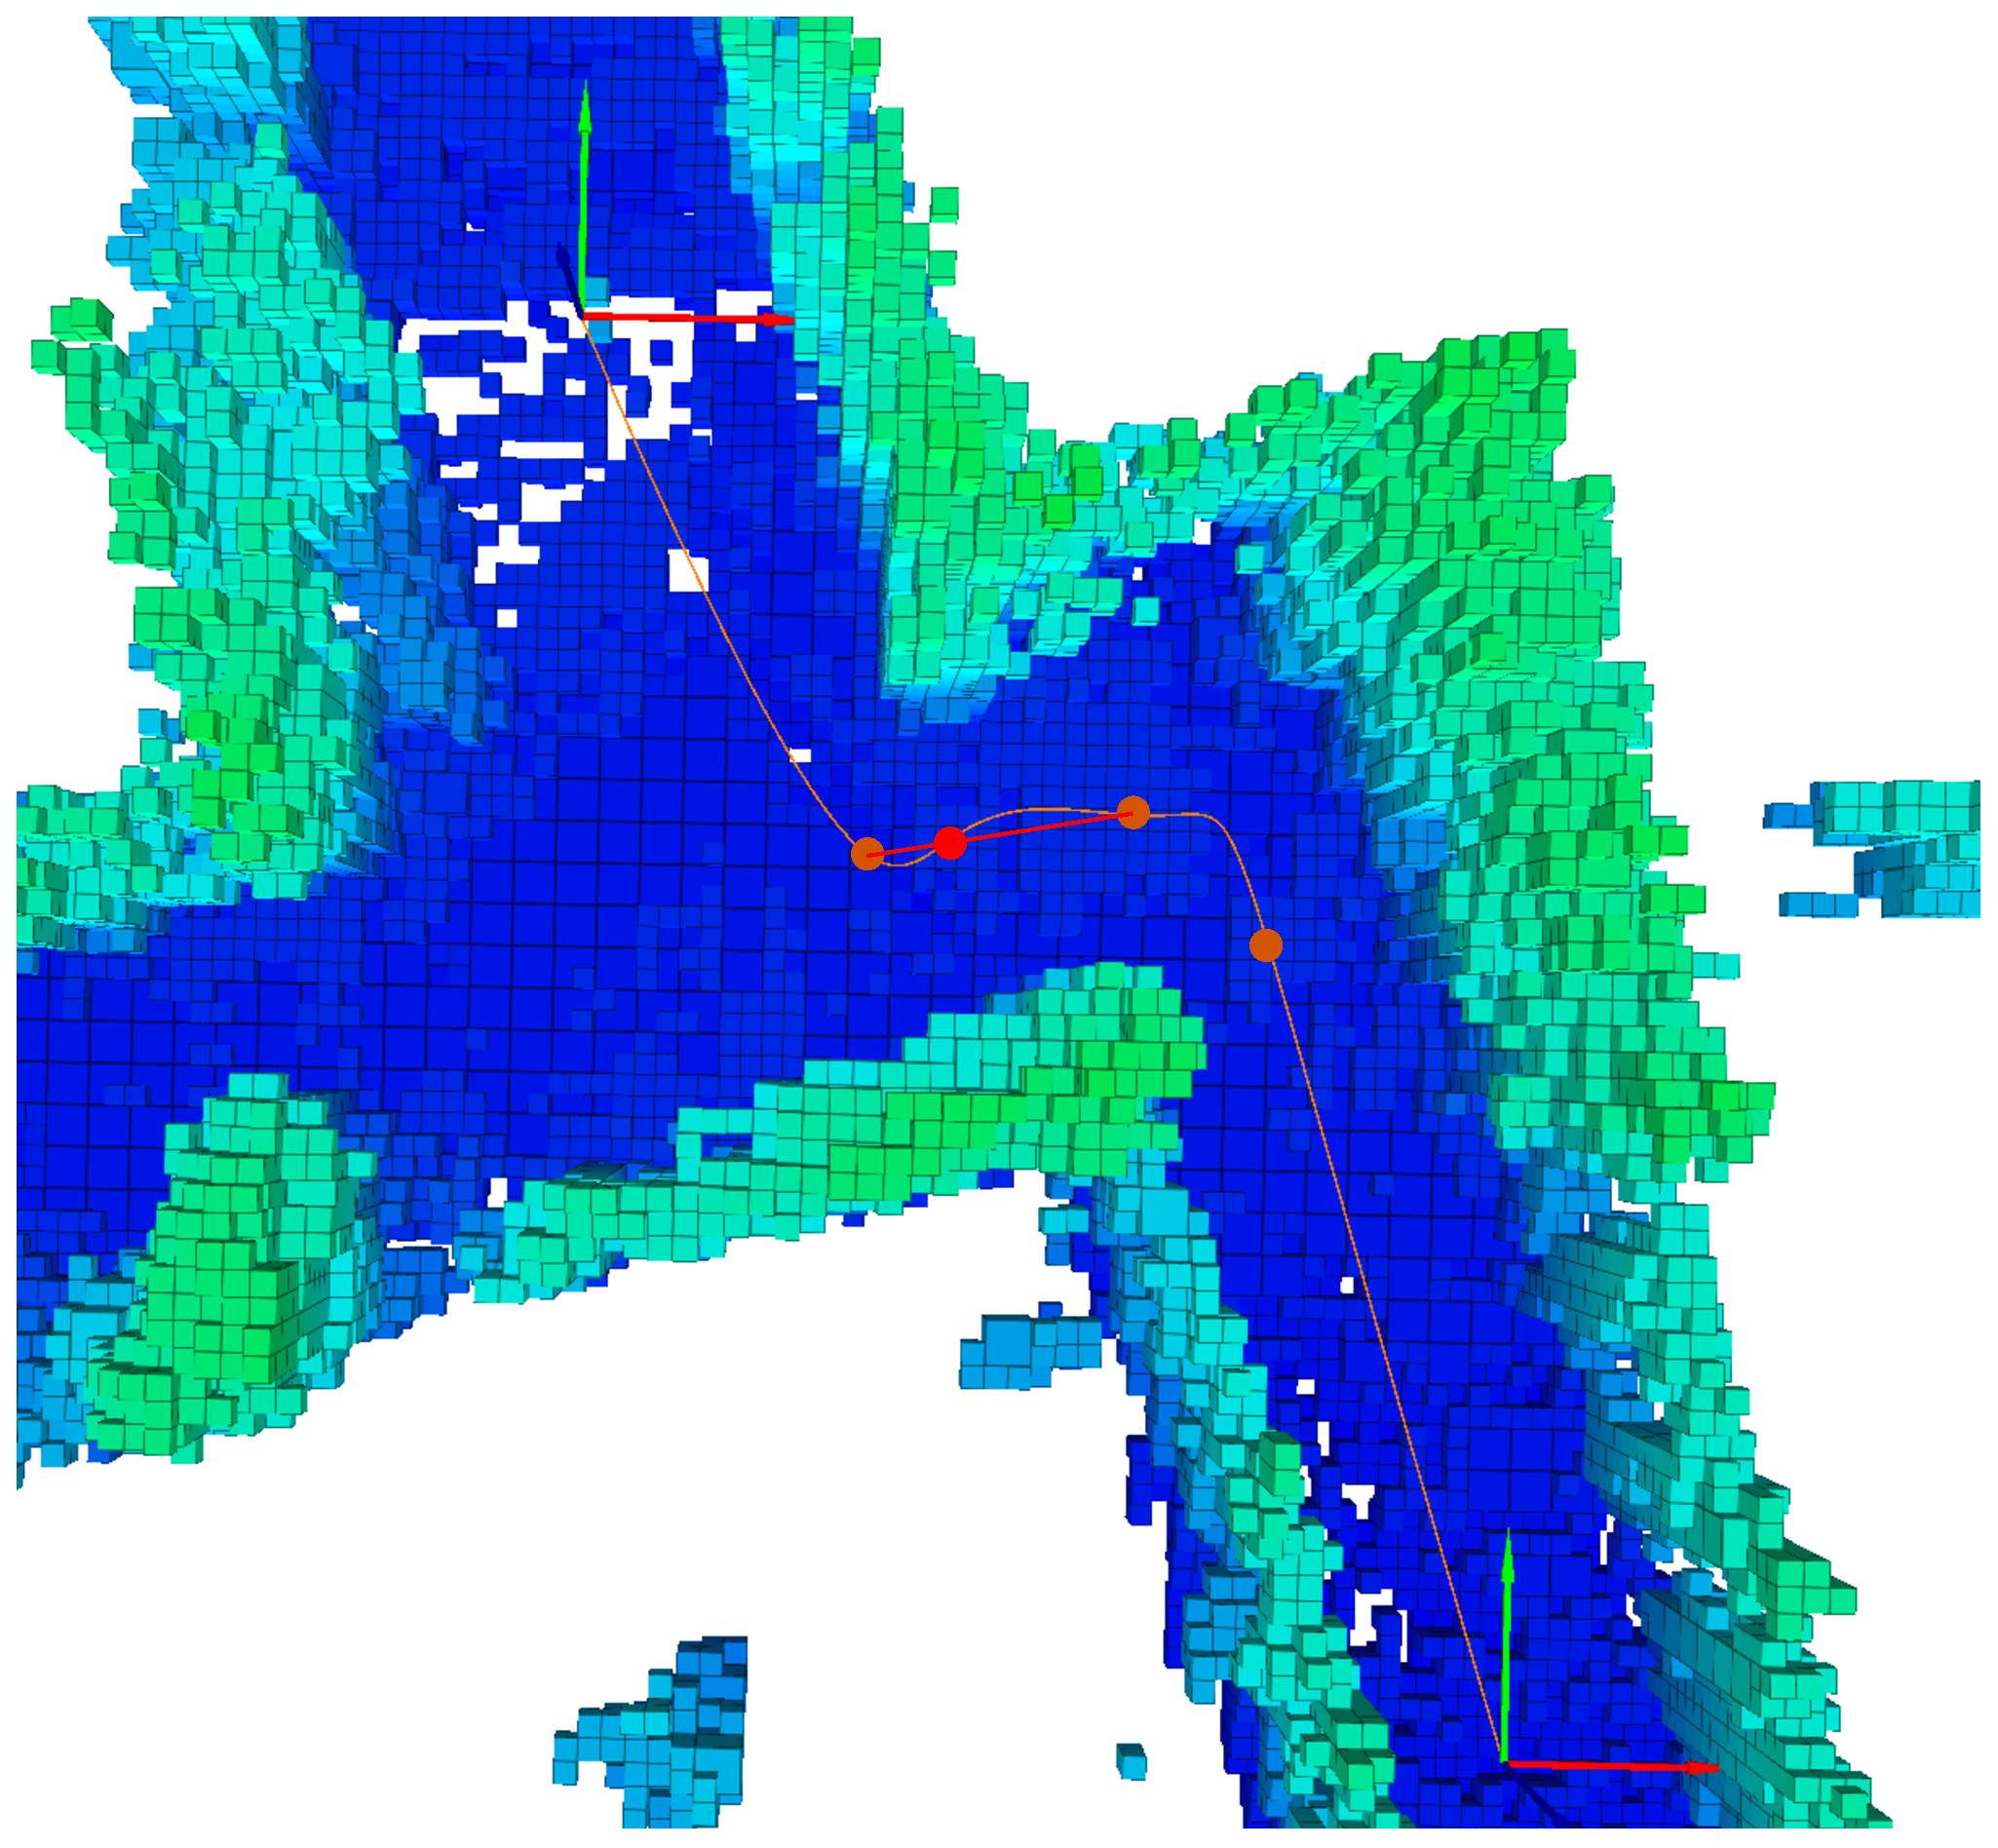
\includegraphics[trim = 45mm 0mm 35mm 0mm, clip,width=1\textwidth]{pics/extensionBLongPred.eps}
   \caption{Polynomial trajectory after a vertex extension.}
\label{pic:RRTstep3}
\end{figure}

As can be seen in figure \ref{pic:RRTstep3} the new vertex is not placed in the middle of the straight line connection. Especially if the segment is long and the collision is close to the start or the end of the segment, placing the new vertex in the middle is not an appropriate approach. To get an idea in which part of the trajectory the collision takes place, the length of the trajectory from the start of the segment to the collision is compared to the total trajectory length in this segment. This ratio is then mapped to the straight line solution and the additional vertex is placed. 
As explained in section \ref{sec:bbx}, the trajectory is in collision as soon as there is any obstacle inside the bounding box. Applied to the trajectory in figure \ref{pic:RRTstepTwo} this means that the collision is detected in the first half of the second segment before the trajectory itself proceeds through the wall of the hallway. Hence, the new vertex in figure \ref{pic:RRTstep3} is closer to the start of the second segment then to the end.



%\begin{figure}[h]
%   \centering
%   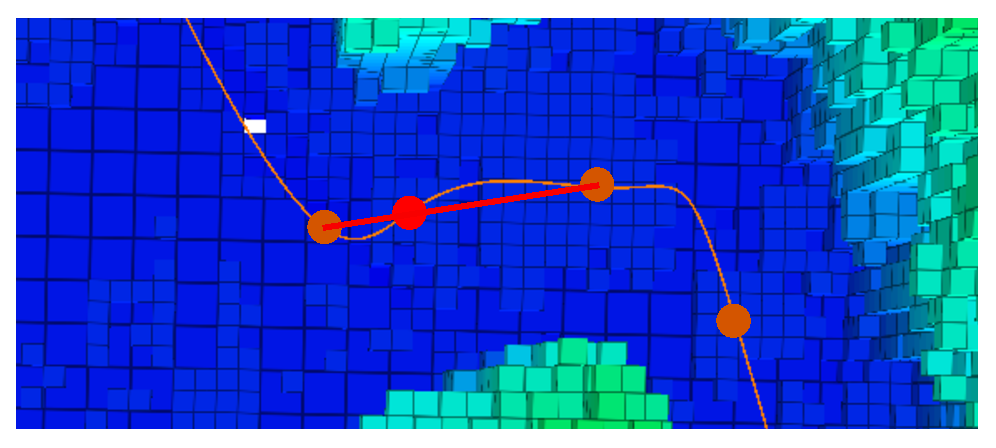
\includegraphics[width=1\textwidth]{pics/extensionBLongPredline.eps}
%   \caption{Ein Bild.}
%\end{figure}



\subsubsection{Perform a nonlinear optimization on the collision-free trajectory.}


\begin{figure}[h]
   \centering
   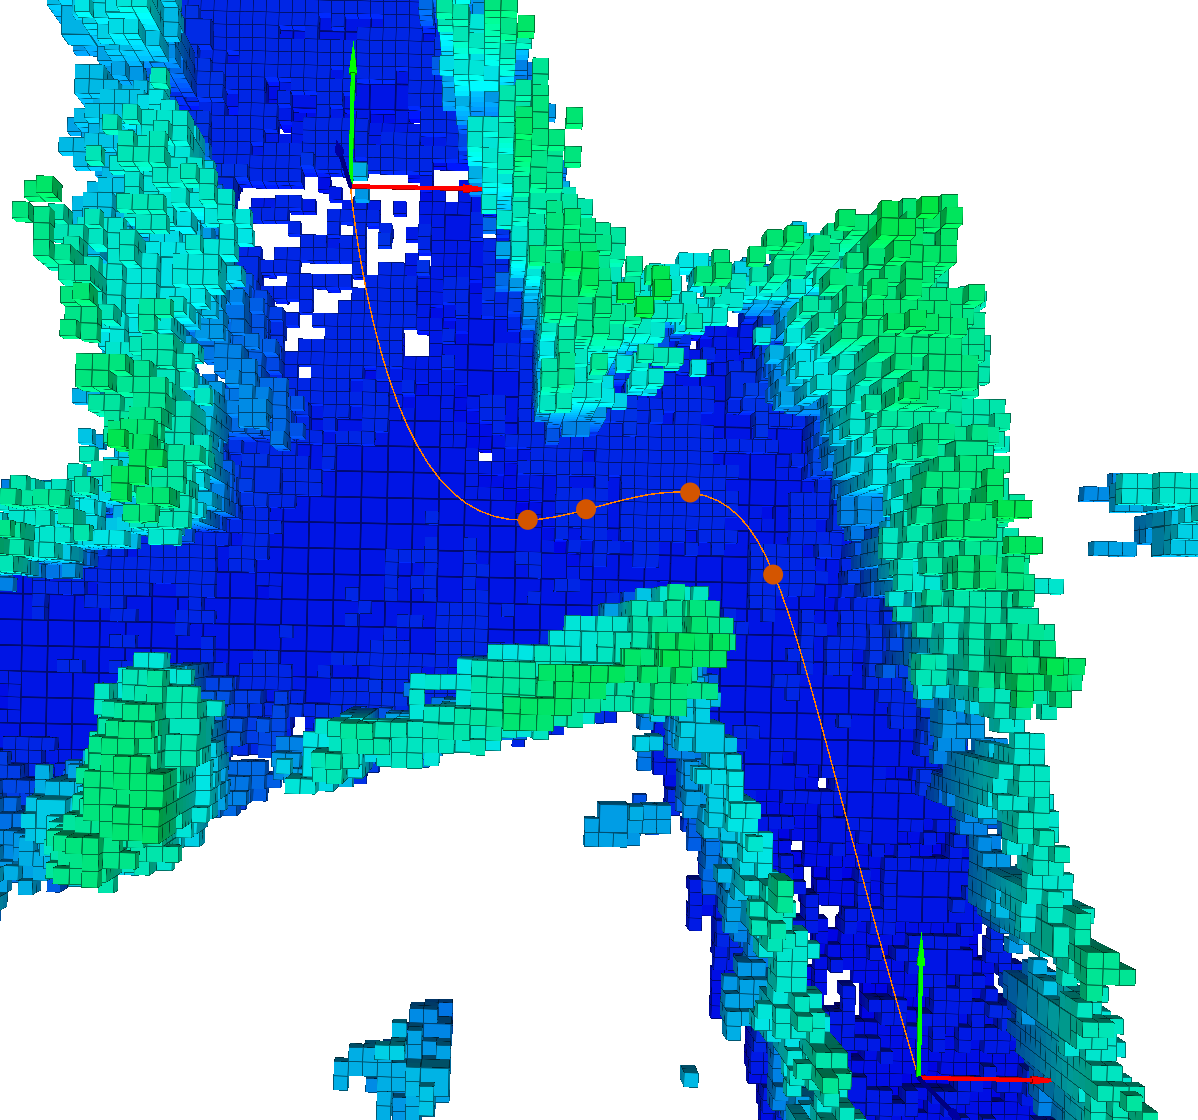
\includegraphics[trim = 45mm 0mm 35mm 0mm, clip,width=1\textwidth]{pics/extensionCLongP.png}
   \caption{Ein Bild.}
\end{figure}




%\subsection{Multiple Vertex Extension}

%\begin{figure}[h]
%   \centering
%   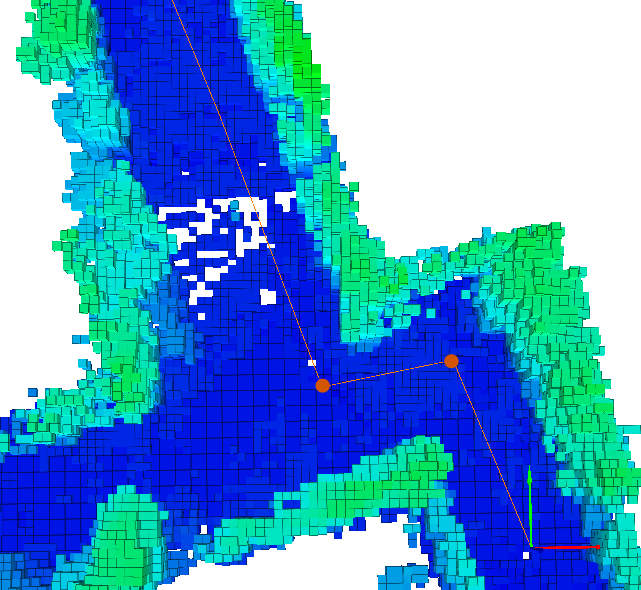
\includegraphics[width=1\textwidth]{pics/1LongP.png}
%   \caption{Ein Bild.}
%\end{figure}
%
%
%
%\begin{figure}[h]
%   \centering
%   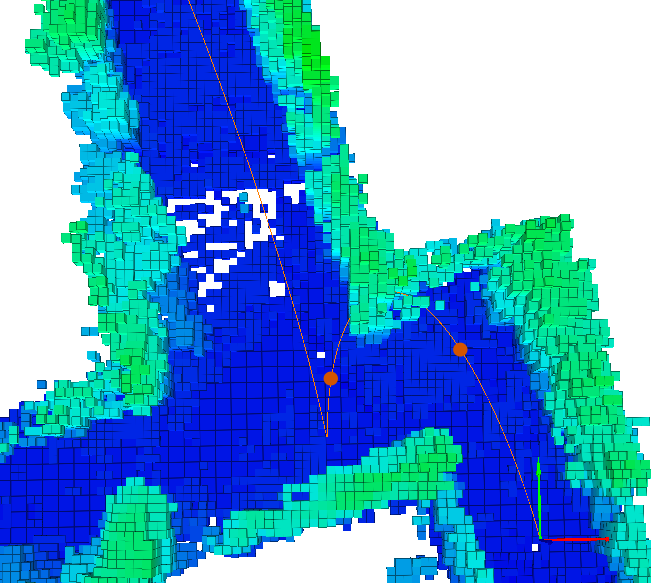
\includegraphics[width=1\textwidth]{pics/1aLongP.png}
%   \caption{Ein Bild.}
%\end{figure}
%
%
%\begin{figure}[h]
%   \centering
%   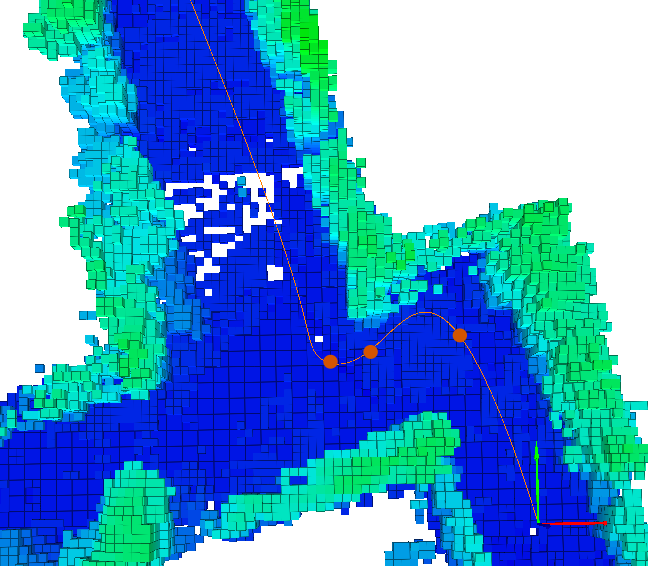
\includegraphics[width=1\textwidth]{pics/1bLongP.png}
%   \caption{Ein Bild.}
%\end{figure}
%
%\begin{figure}[h]
%   \centering
%   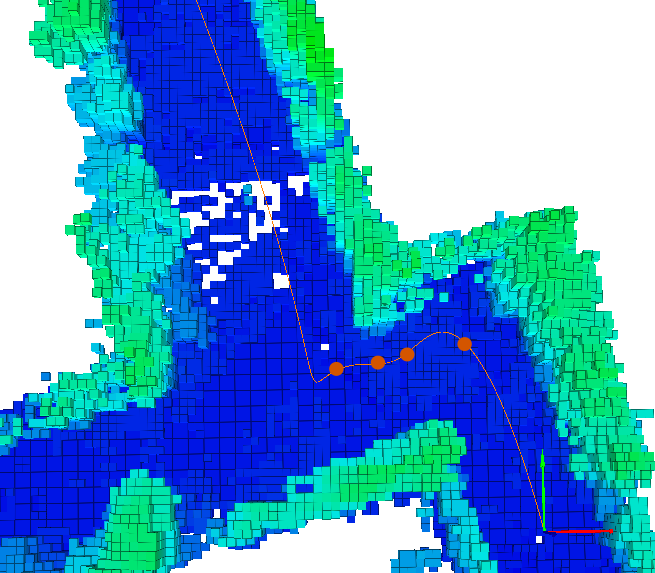
\includegraphics[width=1\textwidth]{pics/1cLongP.png}
%   \caption{Ein Bild.}
%\end{figure}
%
%\begin{figure}[h]
%   \centering
%   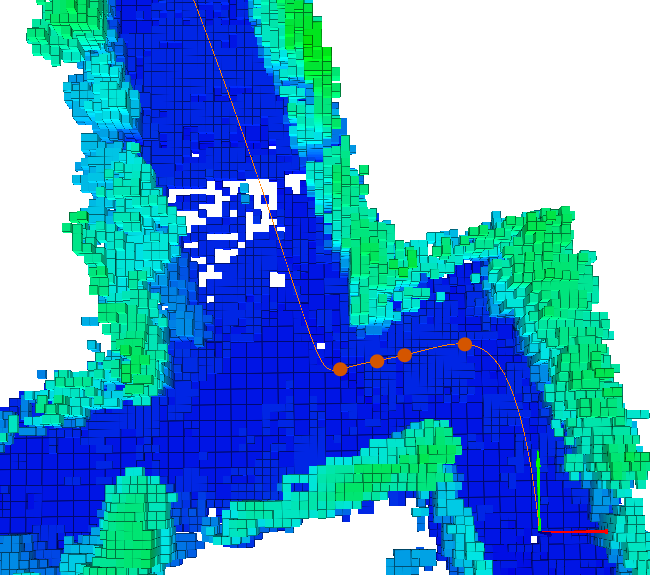
\includegraphics[width=1\textwidth]{pics/1dLongP.png}
%   \caption{Ein Bild.}
%\end{figure}
%
%
%\begin{figure}[h]
%   \centering
%   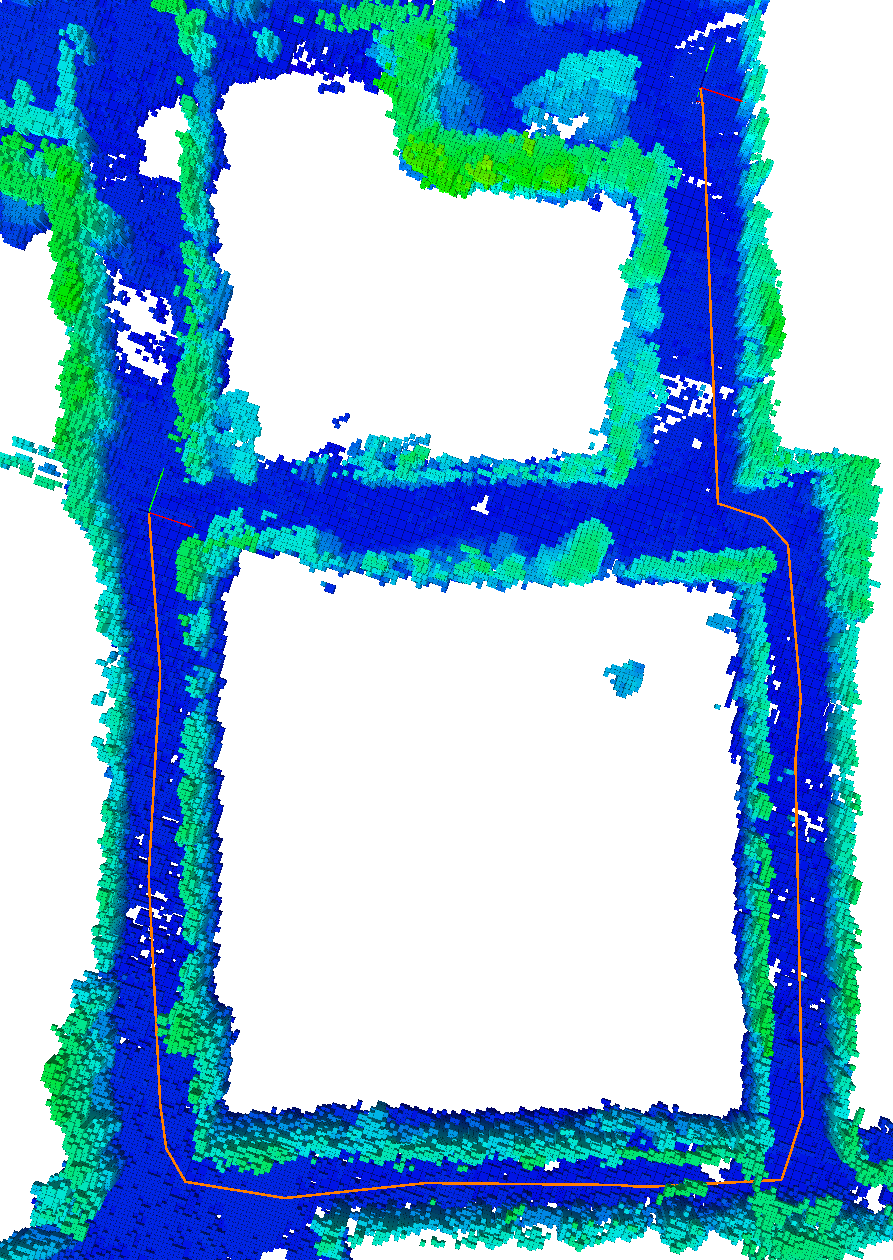
\includegraphics[width=1\textwidth]{pics/MapLine.png}
%   \caption{Ein Bild.}
%\end{figure}
%
%
%\begin{figure}[h]
%   \centering
%   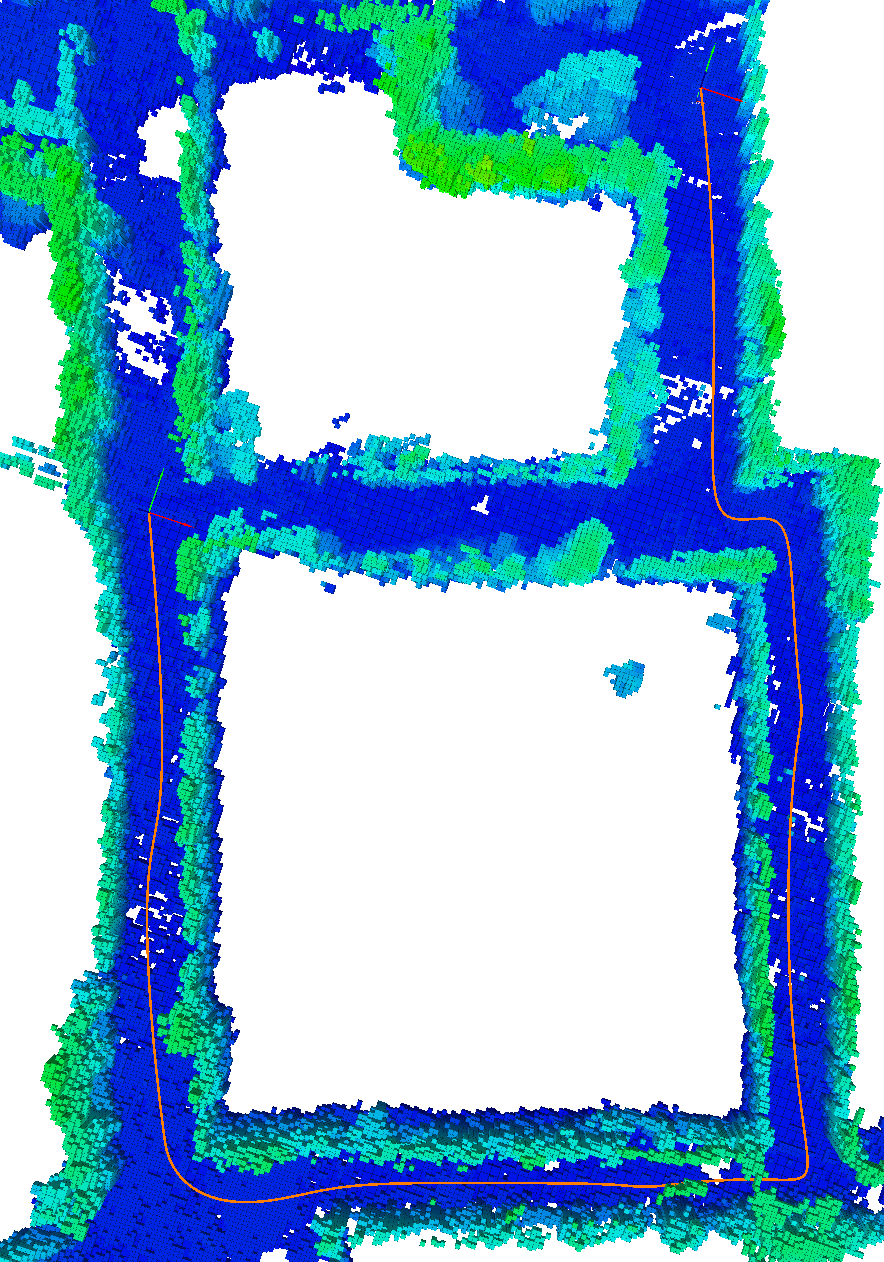
\includegraphics[width=1\textwidth]{pics/MapPoly.png}
%   \caption{Ein Bild.}
%\end{figure}
%
%
%\begin{figure}[h]
%   \centering
%   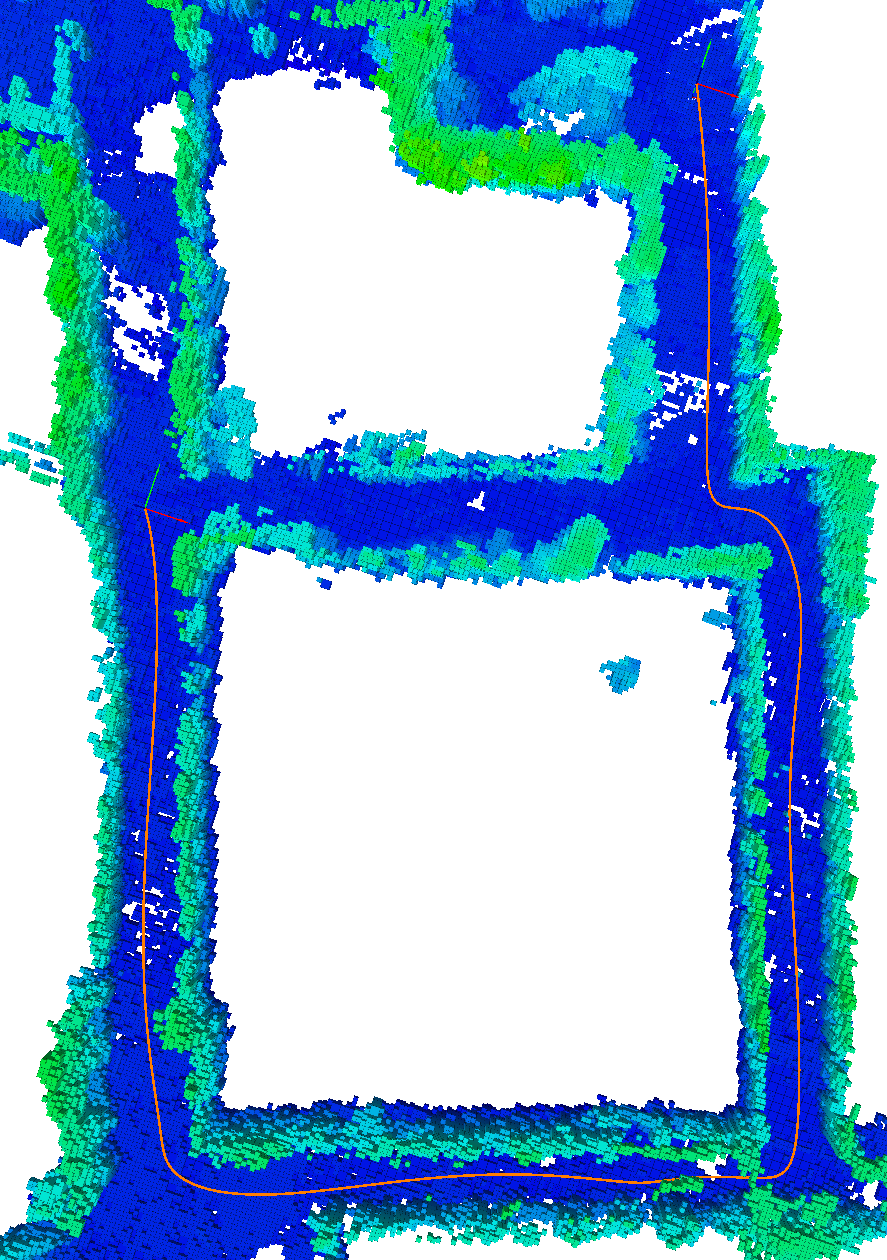
\includegraphics[width=1\textwidth]{pics/MapNlopt.png}
%   \caption{Ein Bild.}
%\end{figure}
